% Options for packages loaded elsewhere
\PassOptionsToPackage{unicode}{hyperref}
\PassOptionsToPackage{hyphens}{url}
\PassOptionsToPackage{dvipsnames,svgnames,x11names}{xcolor}
%
\documentclass[
  man, donotrepeattitle,floatsintext]{apa6}
\usepackage{amsmath,amssymb}
\usepackage{lmodern}
\usepackage{iftex}
\ifPDFTeX
  \usepackage[T1]{fontenc}
  \usepackage[utf8]{inputenc}
  \usepackage{textcomp} % provide euro and other symbols
\else % if luatex or xetex
  \usepackage{unicode-math}
  \defaultfontfeatures{Scale=MatchLowercase}
  \defaultfontfeatures[\rmfamily]{Ligatures=TeX,Scale=1}
\fi
% Use upquote if available, for straight quotes in verbatim environments
\IfFileExists{upquote.sty}{\usepackage{upquote}}{}
\IfFileExists{microtype.sty}{% use microtype if available
  \usepackage[]{microtype}
  \UseMicrotypeSet[protrusion]{basicmath} % disable protrusion for tt fonts
}{}
\makeatletter
\@ifundefined{KOMAClassName}{% if non-KOMA class
  \IfFileExists{parskip.sty}{%
    \usepackage{parskip}
  }{% else
    \setlength{\parindent}{0pt}
    \setlength{\parskip}{6pt plus 2pt minus 1pt}}
}{% if KOMA class
  \KOMAoptions{parskip=half}}
\makeatother
\usepackage{xcolor}
\IfFileExists{xurl.sty}{\usepackage{xurl}}{} % add URL line breaks if available
\IfFileExists{bookmark.sty}{\usepackage{bookmark}}{\usepackage{hyperref}}
\hypersetup{
  pdftitle={Getting a Step Ahead: Using the Regularized Horseshoe Prior to Select Cross-Loadings in Bayesian CFA},
  pdflang={en-EN},
  colorlinks=true,
  linkcolor={Maroon},
  filecolor={Maroon},
  citecolor={Blue},
  urlcolor={blue},
  pdfcreator={LaTeX via pandoc}}
\urlstyle{same} % disable monospaced font for URLs
\usepackage{graphicx}
\makeatletter
\def\maxwidth{\ifdim\Gin@nat@width>\linewidth\linewidth\else\Gin@nat@width\fi}
\def\maxheight{\ifdim\Gin@nat@height>\textheight\textheight\else\Gin@nat@height\fi}
\makeatother
% Scale images if necessary, so that they will not overflow the page
% margins by default, and it is still possible to overwrite the defaults
% using explicit options in \includegraphics[width, height, ...]{}
\setkeys{Gin}{width=\maxwidth,height=\maxheight,keepaspectratio}
% Set default figure placement to htbp
\makeatletter
\def\fps@figure{htbp}
\makeatother
\setlength{\emergencystretch}{3em} % prevent overfull lines
\providecommand{\tightlist}{%
  \setlength{\itemsep}{0pt}\setlength{\parskip}{0pt}}
\setcounter{secnumdepth}{-\maxdimen} % remove section numbering
% Make \paragraph and \subparagraph free-standing
\ifx\paragraph\undefined\else
  \let\oldparagraph\paragraph
  \renewcommand{\paragraph}[1]{\oldparagraph{#1}\mbox{}}
\fi
\ifx\subparagraph\undefined\else
  \let\oldsubparagraph\subparagraph
  \renewcommand{\subparagraph}[1]{\oldsubparagraph{#1}\mbox{}}
\fi
\newlength{\cslhangindent}
\setlength{\cslhangindent}{1.5em}
\newlength{\csllabelwidth}
\setlength{\csllabelwidth}{3em}
\newlength{\cslentryspacingunit} % times entry-spacing
\setlength{\cslentryspacingunit}{\parskip}
\newenvironment{CSLReferences}[2] % #1 hanging-ident, #2 entry spacing
 {% don't indent paragraphs
  \setlength{\parindent}{0pt}
  % turn on hanging indent if param 1 is 1
  \ifodd #1
  \let\oldpar\par
  \def\par{\hangindent=\cslhangindent\oldpar}
  \fi
  % set entry spacing
  \setlength{\parskip}{#2\cslentryspacingunit}
 }%
 {}
\usepackage{calc}
\newcommand{\CSLBlock}[1]{#1\hfill\break}
\newcommand{\CSLLeftMargin}[1]{\parbox[t]{\csllabelwidth}{#1}}
\newcommand{\CSLRightInline}[1]{\parbox[t]{\linewidth - \csllabelwidth}{#1}\break}
\newcommand{\CSLIndent}[1]{\hspace{\cslhangindent}#1}
\ifLuaTeX
\usepackage[bidi=basic]{babel}
\else
\usepackage[bidi=default]{babel}
\fi
\babelprovide[main,import]{english}
% get rid of language-specific shorthands (see #6817):
\let\LanguageShortHands\languageshorthands
\def\languageshorthands#1{}
% This preamble allows to remove the redundant title page from papaja's output.pdf
\usepackage{atbegshi}% http://ctan.org/pkg/atbegshi
\AtBeginDocument{\AtBeginShipoutNext{\AtBeginShipoutDiscard}}
% Manuscript styling
\usepackage{upgreek}
\captionsetup{font=singlespacing,justification=justified}

% Table formatting
\usepackage{longtable}
\usepackage{lscape}
% \usepackage[counterclockwise]{rotating}   % Landscape page setup for large tables
\usepackage{multirow}		% Table styling
\usepackage{tabularx}		% Control Column width
\usepackage[flushleft]{threeparttable}	% Allows for three part tables with a specified notes section
\usepackage{threeparttablex}            % Lets threeparttable work with longtable

% Create new environments so endfloat can handle them
% \newenvironment{ltable}
%   {\begin{landscape}\centering\begin{threeparttable}}
%   {\end{threeparttable}\end{landscape}}
\newenvironment{lltable}{\begin{landscape}\centering\begin{ThreePartTable}}{\end{ThreePartTable}\end{landscape}}

% Enables adjusting longtable caption width to table width
% Solution found at http://golatex.de/longtable-mit-caption-so-breit-wie-die-tabelle-t15767.html
\makeatletter
\newcommand\LastLTentrywidth{1em}
\newlength\longtablewidth
\setlength{\longtablewidth}{1in}
\newcommand{\getlongtablewidth}{\begingroup \ifcsname LT@\roman{LT@tables}\endcsname \global\longtablewidth=0pt \renewcommand{\LT@entry}[2]{\global\advance\longtablewidth by ##2\relax\gdef\LastLTentrywidth{##2}}\@nameuse{LT@\roman{LT@tables}} \fi \endgroup}

% \setlength{\parindent}{0.5in}
% \setlength{\parskip}{0pt plus 0pt minus 0pt}

% \usepackage{etoolbox}
\makeatletter
\patchcmd{\HyOrg@maketitle}
  {\section{\normalfont\normalsize\abstractname}}
  {\section*{\normalfont\normalsize\abstractname}}
  {}{\typeout{Failed to patch abstract.}}
\patchcmd{\HyOrg@maketitle}
  {\section{\protect\normalfont{\@title}}}
  {\section*{\protect\normalfont{\@title}}}
  {}{\typeout{Failed to patch title.}}
\makeatother
\shorttitle{Using the RHSP to Select Cross-Loadings in Bayesian CFA}
\keywords{\newline\indent Word count: X}
\DeclareDelayedFloatFlavor{ThreePartTable}{table}
\DeclareDelayedFloatFlavor{lltable}{table}
\DeclareDelayedFloatFlavor*{longtable}{table}
\makeatletter
\renewcommand{\efloat@iwrite}[1]{\immediate\expandafter\protected@write\csname efloat@post#1\endcsname{}}
\makeatother
\usepackage{csquotes}
\ifLuaTeX
  \usepackage{selnolig}  % disable illegal ligatures
\fi

\title{Getting a Step Ahead: Using the Regularized Horseshoe Prior to Select Cross-Loadings in Bayesian CFA}
\author{\phantom{0}}
\date{}


\affiliation{\phantom{0}}

\begin{document}
\maketitle

\thispagestyle{empty}

\begin{large}
\noindent Research Master's programme 
Methodology and Statistics for the Behavioural, Biomedical and Social Sciences \newline
Utrecht University, the Netherlands \newline
\newline
\newline
\newline
\newline
MSc Thesis Johannes Michael Benjamin Koch (6412157) 
\newline
TITLE: "Getting a Step Ahead: Using the Regularized Horseshoe Prior to Select Cross-Loadings in Bayesian CFA"
\newline
June 2022 
\newline
\newline
\newline
\newline
\newline
Supervisor:\newline
Dr. Sara van Erp \newline
\newline
\newline
Second grader: \newline
Dr. Beth Grandfield
\newline
\newline
\newline
\newline
Preferred journal of publication: Structural Equation Modeling
\newline
Word count: 9465
\newline
\end{large}
\addtocounter{page}{-1}
\clearpage
\pagebreak

% make page numbers start from second page 
%\pagenumbering{arabic}
%\setcounter{page}{0}
%\thispagestyle{empty}
% make page numbers from second page 
\pagestyle{plain}

\clearpage

\hypertarget{abstract}{%
\section{Abstract}\label{abstract}}

This is the first study to compare the Regularized Horseshoe Prior (RHSP) to the Small Variance Normal Prior (SVNP) in their performance in regularizing cross-loadings in Bayesian CFA. The SVNP can be used to shrink cross-loadings in CFA to(wards) zero to identify models. This often results in biased model estimates, as also large cross-loadings are shrunken substantially. The RHSP was expected to regularize cross-loadings more efficiently, avoiding the bias of the SVNP, by allowing large cross-loadings to escape shrinkage within a single estimation step. It was found that indeed the SVNP had overall higher levels of bias than the RHSP under the presence of large cross-loadings. Hereby, the RHSP was robust across sample sizes, and different hyper-parameter settings, although under some convergence failed. Regarding the Power and Type-I-Error rate in selecting cross-loadings as non-zero, both priors performed poorly, which is partially explained by the low sample sizes considered.

\hypertarget{introduction}{%
\section{Introduction}\label{introduction}}

The art of statistical modeling revolves around coming up with an appropriate simplification, a \emph{model}, of a true \emph{data-generating process}. Hereby, a fundamental trade-off between model simplicity and model complexity arises, that is mostly known as \emph{bias-variance trade-off}. Simple models with few parameters have high bias, meaning that they deviate substantially from the true data-generating process, and low variance, such that they generalize well to other datasets from the same population. Complex models with large numbers of parameters tend to have low bias and high variance. They are thus prone to over-fitting, i.e.~picking up patterns that are only relevant in the dataset at hand, but do not generalize well to other datasets. Moreover, complex models can be cumbersome to interpret and often a large number of observations is required to estimate them (Cox, 2006; James, Witten, Hastie, \& Tibshirani, 2021).

In confirmatory factor analysis (CFA, Bollen, 1989) it is common practice to deal with the bias-variance trade-off in a brute-force manner, by imposing a so-called simple structure. Here, cross-loadings, factor loadings that relate items to factors that they
theoretically do not belong to, are fixed to zero to yield an identified and easy-to-interpret model. This often leads to poor model fit, which forces researchers to free some cross-loadings after the fact based on empirical grounds (modification indices) to improve fit. This procedure is flawed, as it risks capitalization on chance and thereby over-fitting (MacCallum, Roznowski, \& Necowitz, 1992).

As a Bayesian solution to this issue Muthén and Asparouhov (2012) proposed identifying CFA models, by setting the so-called \emph{Small Variance Normal Prior} (SVNP) for cross-loadings, which is a normal distribution with mean zero and a very small variance (e.g.~\(\sigma^2\) = 0.01). This prior attaches large prior mass to cross-loadings of or near zero, while attaching almost no prior mass to cross-loadings further from zero, such that all cross-loadings in the model are shrunken. However, shrinking also those cross-loadings that are further from zero substantially introduces bias to the model (Lu, Chow, \& Loken, 2016). Consequently, Bayesian CFA requires a two-step approach. First, the model is estimated with the SVNP set for the cross-loadings and cross-loadings are selected as non-zero when their 95\% credible intervals does not contain zero (Muthén \& Asparouhov, 2012). The model is then re-estimated, where cross-loadings that have been selected to be non-zero are freely estimated without shrinkage, and the remaining cross-loadings are fixed to zero, avoiding the bias in the model of the previous step. Correctly selecting cross-loadings as non-zero can pose a challenge in practice, as the performance of different selection criteria depends on a broad set of conditions, making it difficult to formulate general recommendations for researchers (Zhang, Pan, \& Ip, 2021). It is thus desirable to identify shrinkage-priors that can regularize CFA models without causing substantial bias, within a single step.

One promising regularization-prior that can be expected to allow estimating CFA models with less bias within a single step is the so-called Regularized Horseshoe Prior (RHSP), which is designed to let large parameters escape shrinkage. While the Regularized Horseshoe Prior has been shown to perform excellently in the selection of relevant predictors in regression (Piironen \& Vehtari, 2017b; Van Erp, Oberski, \& Mulder, 2019), no previous research has validated its performance in regularizing cross-loadings in CFA. We therefore aim to compare the RHSP to the SVNP in their performance in regularizing cross-loadings in Bayesian CFA.

\hypertarget{theoretical-background}{%
\section{Theoretical Background}\label{theoretical-background}}

\hypertarget{regularization}{%
\subsection{Regularization}\label{regularization}}

A classic method of trying to find a balance between model complexity and model simplicity is \emph{regularization} (Hastie, Tibshirani, \& Wainwright, 2015). Regularization entails adding some bias to a model on purpose to reduce its variance. This helps to make models easier to interpret and more generalizable. In a frequentist context, regularization is achieved by adding a so-called penality term to the cost function of a model. This ensures that model parameters that are irrelevant, e.g.~small regression coefficients in a regression model with a large number of predictors, are shrunken to (or towards) zero. For a regression model, where we predict the scores of i, \ldots, N individuals on an outcome \(y_i\) based on scores on a vector of predictors \(x_i\), the vector of regression coefficients \(\beta\), and a random error term \(e_i\):
\[y_i = \beta \mathbf{x_i} + e_i, \ where \]
\[e_i \sim \mathcal{N}(0, \sigma^2), \]
the Ordinary Least Squared Residuals estimates of \(\beta\) are obtained by minimizing the sum of squared residuals:
\[ \hat{\beta} = \underset{\beta}{argmin} \{ \Sigma_{i=1}^N(y_i - \beta\mathbf{x_{i}} )^2 \}.\] Penalized regression adds a a penalty term to this cost function, which is generally denoted as \(||\beta||_L\):
\[ \hat{\beta} = \underset{\beta}{argmin} \{ \Sigma_{i=1}^N(y_i - \beta \mathbf{x_{i}} )^2 + \lambda ||\beta||_{L} \}.\]
When L = 1, the so-called L-1 norm, \(||\beta||_1 = \Sigma_{j=1}^p |\beta_j|\). This is the well-known LASSO penality (Tibshirani, 1996, 2011). Here, the absolute value of the regression coefficients are added up, multiplied by \(\lambda\) , and then added to the sum of the squared error within the model's cost-function. The basic intuition is as follows. Just as minimizing sum of the (squared residuals) leads to estimates of the model parameters with minimally small residuals, minimizing the (absolute) sum of the regression coefficients results in smaller values of the regression coefficients. Hereby, the larger \(\lambda\), the more weight the penalty has, and thereby the higher the amount of shrinkage to(wards) zero. When, L = 2, the L2-norm, \(||\beta||_2 = \sqrt{\Sigma_{j=1}^p \beta_j^2}\). This is the famous ridge penalty (Hoerl \& Kennard, 2000). Here, the same general principle is followed, with this time not the absolute, but the Square Root of the sum of squares of the regression coefficients being minimized. In practice, one key difference between the LASSO and the ridge penalty is that the former shrinks some coefficient entirely to zero (thereby actively selecting predictors), whereas in ridge regression coefficients are only shrunken approximately but never entirely to zero.

Regularization can also be applied for more complex models, which is illustrated by the large body of literature applying regularization in in Structural Equation Modeling. Regularized SEM entails adding penalties to the cost function of SEM models (typically a variant of the maximum likelihood cost function) to reach sparser models. In SEM models a large variety of parameters exist for which it is desirebale to possess succesful selection methods. Regularizd SEM has been applied to successfully select cross-loadings and residual covariances in CFA, especially under favorable conditions such as large sample sizes. (Jacobucci, Grimm, \& McArdle, 2016). Also structural model parameters, such as regression coefficients in MIMIC (Jacobucci, Brandmaier, \& Kievit, 2019; Jacobucci et al., 2016), or indirect effects in mediation models with continuous (Serang, Jacobucci, Brimhall, \& Grimm, 2017) or dichotomous outcomes (Serang \& Jacobucci, 2020), have successfully been regularized through the usage of adjusted penality functions, mimicking the LASSO or ridge penalites in regression, outlined above.
- Multigroup modeling {[}lindstrom\_model\_2020; Muthen and Asparouhov (2013){]}

\begin{itemize}
\tightlist
\item
  Lasso:
  Chen, Guo, Zhihan, Zhang, Lijin, and Pan, Junhao (2021)

  \begin{enumerate}
  \def\labelenumi{\arabic{enumi}.}
  \tightlist
  \item
    Guo, Zhu, Chow, and Ibrahim (2012) non parametric SEM;
  \end{enumerate}
\end{itemize}

One key disadvantage of the frequentist regularization approach is that it depends on optimization. With more complicated penalties, and in particular for complex models, it can be hard to derive optimizable cost functions in practice. Also the derivation of unbiased standard errors is often challenging under such circumstances, which hinders reliable inference (Jacobucci \& Grimm, 2018; Jacobucci et al., 2016). Bayesian approaches to regularization overcome these obstacles (Jacobucci \& Grimm, 2018). In Bayesian model estimation, the so-called Joint Posterior Distribution of the model-parameters given the data \(P({\theta} | data)\) is a combination of the data and the prior. Priors can therefore be used to shrink model-parameter estimates to(wards) zero, which is then called a shrinkage-prior. In the most simple case one can simply set a normal prior for parameters that is centered around zero, which resembles the ridge-penalty (Hsiang, 1975). The lasso penalty can be mimicked by setting a Laplace- (double exponential) prior for parameters (HANS, 2009; Park \& Casella, 2008; see Van Erp et al., 2019 for the Bayesian equivalents of other relevant penalties). The fact that in Bayesian inference the whole joint posterior distribution of the model parameters can be sampled by means of MCMC methods poses a key advantage. This renders it unnecessary to derive standard errors, as the variance of the posterior is directly available. Also complex shrinkage-priors can be implented without having to yield an optimizable cost-function, making Bayesian regularization a very flexible approach.

\hypertarget{bayesian-cfa-the-small-variance-normal-prior-svnp}{%
\subsection{Bayesian CFA: The Small Variance Normal Prior (SVNP)}\label{bayesian-cfa-the-small-variance-normal-prior-svnp}}

Confirmatory Factor Analysis (CFA, Bollen, 1989) is an essential tool for modeling measurement structures, falling under the class of Structural Equation Modeling (SEM). For every individual i, the scores on a vector of p observed indicators \(\mathbf{y}_i\) (typically items of a psychological test):
\[\boldsymbol{y}_i = \boldsymbol{\mu} + \Lambda \boldsymbol{\eta}_i + \boldsymbol{e}_i ,\]
where \(\boldsymbol{y}_i\) is a \(p \times 1\) vector of observed indicators, \(\boldsymbol{\mu}\) is a \(p \times 1\) vector of intercepts, \(\Lambda\) is a \(p \times q\) matrix of factor loadings, \(\boldsymbol{\eta}_i\) is a \(q \times 1\) vector of scores on the q latent factors, and \(\boldsymbol{e}_i\) is a \(p \times 1\) is a random vector of random (measurement) error terms. Here, \(\Lambda\) is thus the part of the equation that relates the latent variables to the observed scores on the items.

We can differentiate between so-called main-loadings, and cross-loadings. The former are factor loadings that relate factor and items to one another that are theoretically expected to have a relationship. Cross-loadings are factor loadings that relate factors to items between which, theoretically, no relationship should exist. One key property of CFA is that a clear expectation on the factor structure, i.e.~which factor loads on which items, is assumed. This allows to formulate clear expectations on which items can be viewed as cross-loadings. Consequently, a natural way of identifying

\begin{itemize}
\item
  natural way of identyfing fixing cross-loadings to zero
\item
  This on top of other identification methods
\item
  In practice models allow for some cross-loaingd to be non-zero, depening on a number of factors
\item
  often ppor model fit , modification indicies \textgreater{} however not without problems (elaborate)
\item
  alternative approach Muthen:
\item
  fixing to zero =
\item
\item
  However: Problem\textgreater{} bias
\end{itemize}

First, bias naturally occurs in the large cross-loadings itself. However, also in other parameters, such as factor-correlations or main-loadings, substantial bias can arise, as they are estimated conditionally on the cross-loadings.
- 2 step approach:

Bayesian LASSO

\hypertarget{the-spike-and-slab-prior}{%
\subsection{The Spike and Slab Prior}\label{the-spike-and-slab-prior}}

One suitable regularization prior for the purpose of selecting cross-loadings in
regularized Bayesian SEM is the so-called Spike-and-Slab Prior (George \& McCulloch, 1993; Ishwaran \& Rao, 2005; Mitchell \& Beauchamp, 1988). This prior is a discrete mixture of an extremely peaked prior around zero (the spike), and a very flat prior for larger parameters (the slab). Formally, and applied to the cross-loadings in CFA, for every Cross-loading of factor j
on item k, the Spike-and-Slab Prior can be specified as (Lu et al., 2016):
\[\lambda_{c,jk} |r_{jk} \sim (1 \ - \ r_{jk})\delta_0 + r_{jk} \mathcal{N}(0, c^2_{jk}) , \ with\]
\[r_{jk} \sim \mathcal{Bernoulli}(p_{jk}).\]
The basic intuition is as follows. When \(r_{jk} = 1\), \(\lambda_{c,jk} \sim \mathcal{N}(0, c^2_{jk})\), hence \(\lambda_{c,jk}\) is assigned to the slab. When \(r_{jk} = 0\), \(\lambda_{c,jk} \sim \delta_0\), and is thus assigned to the spike. This ensures that large cross-loadings, that are are relevant are not shrunken while small, negligible cross-loadings are shrunken to zero.

Lu et al.~(2016) found that this prior is performing well in shrinking truly zero cross-loadings to zero, while not shrinking (relevant) large cross-loadings to avoid bias, especially under favorable conditions with large sample sizes and cross-loadings. However, the Spike and Slab Prior cannot be implemented in STAN, one of the most popular package for MCMC-sampling, as STAN does not allow for discrete mixture priors (Betancourt, 2018; Stan Development Team, 2021). This calls for a \emph{non-discrete} alternative shrinkage-prior that also outperforms the SVNP within a single estimation step.

\hypertarget{the-regularized-horseshoe-prior-rhsp}{%
\subsection{The Regularized Horseshoe Prior (RHSP)}\label{the-regularized-horseshoe-prior-rhsp}}

A fully continuous alternative to the Spike and Slab prior that is implementable in STAN is the so-called \emph{Regularized Horseshoe Prior} (RHSP, Piironen \& Vehtari, 2017a, 2017b). This prior is an extension of the Horseshoe Prior (Carvalho, Polson, \& Scott, 2010). The main idea of the original Horseshoe Prior is that there is a \emph{global shrinkage parameter} \(\tau\), shrinking all cross-loadings to zero. Next to this, there is a \emph{local shrinkage parameter} \(\bar{\omega}_{jk}\)\footnote{We deviate from the common notation of the local shrinkage parameter as \(\bar{\lambda}\), as this letter is commonly used to denote factor loadings in CFA.} that allows truly large cross-loadings to escape the shrinkage, by setting thick Cauchy tails for the local scales \(\omega_{jk}\) (Polson \& Scott, 2010). Formally, the Horseshoe prior for every cross-loading of factor j on item k is specified as follows:
\[\lambda_{c,jk} | \omega_{jk}, \tau, c\sim \mathcal{N}(0, \ \omega^2_{jk} \tau^2), \ where\]
\[\omega_{jk} \sim \mathcal{C^+}(0, 1).\]
The name-giving intuition behind the horseshoe prior becomes clear when considering the finding that a so-called shrinkage factor \(k_{jk}\) can be derived for the individual cross-loadings (Carvalho et al., 2010; Piironen \& Vehtari, 2017b). This shrinkage factor ranges from zero to one, with zero meaning no, and one meaning a lot of shrinkage. When plotting the density of \(k_{jk}\) there is a very high peak at at very low values and a very high peak of high values, resulting in a plot that resembles a horseshoe, illustrating that the Horseshoe Prior has the desired property of either shrinking parameters very little, or very much, with very few parameters that are shrunken in a non-extreme fashion.

The Horseshoe Prior was found consistently to possess the theoretical properties of not shrinking large parameters while shrinking small parameters substantially to zero, in practice (Carvalho et al., 2010; Datta \& Ghosh, 2013; Polson \& Scott, 2010; Van Der Pas, Kleijn, \& Van Der Vaart, 2014). However, due to its Cauchy tails it suffers from the same issues as a Cauchy prior. Specifically, not shrinking large parameters at all can lead to estimation issues, especially when parameters are weakly identified. This happens for instance in logistic regression with separable data, where a flat likelihood and thereby a weakly identified model arises (Ghosh, Li, \& Mitra, 2018). The RHSP prevents such issues by shrinking also large parameters a little bit. For every cross-loading of factor j on item k:
\[\lambda_{c,jk} | \bar{\omega}_{jk}, \tau, c\sim \mathcal{N}(0, \ \bar{\omega}^2_{jk} \tau^2), \ with \ \bar{\omega}^2_{jk} = \frac{c^2\omega_{jk}^2}{c^2 + \tau^2 \omega_{jk}^2},\]
\[\tau | df_{global}, s_{global} \sim half-t_{df_{global}}(0,\  s_{global}^2), \ with \  s_{global} = \frac{p_0}{p-p_0}\frac{\sigma}{\sqrt{N}},\]
\[\omega_{jk}| df_{local}, s_{local} \sim half-t_{df_{local}}(0, \ s_{local}^2),\]
\[c^2 | df_{slab}, s_{slab} \sim \mathcal{IG}(\frac{df_{slab}}{2}, \  df_{slab} \times \frac{s_{slab}^2}{2}),\]
where \(p_0\) represents a prior guess of the number of relevant cross-loadings. It is not necessary to use \(p_0\). One can simply set \(s_{global}\) manually, whereby it is worth to consider that a \(s_{global}\) created based on a \(p_0\) will typically be much lower than 1 (Piironen \& Vehtari, 2017b). Note that we specify the RHSP in its most general form. Setting the degrees of freedoms of the half-t-distributions to 1 results in half-Cauchy distributions. Strictly speaking, the prior is only a Regularized \emph{Horseshoe} Prior when this is the case. In the current study we vary the degrees of freedoms of all scale parameters to assess the extent to which the sparcifying properties as well as the convergence of the RHSP are influenced by these parameters.

The intuition of how the RHSP shrinks large parameters a little bit is best illustrated by assuming that c is a given constant. Now, when \(\tau^2 \omega^2_{jk} < c^2\), \(\bar{\omega}^2_{jk} \to \omega^2_{jk}\). Hence, in this case the RHSP approaches the original Horseshoe Prior, with equally pronounced shrinkage to zero. In the limit, the product of \(\tau^2\) and \(\omega^2_{jk}\) will be smaller under small cross-loadings. Datasets coming from a population with a true small cross-loading should, on average, possess the property of steering the posterior estimates towards small values of the local shrinkage factor, which allows these parameters to escape the shrinkage. However, when \(\tau\) is far from zero, hence under large true cross-loadings, \(\tau^2 \omega^2_{jk} > c^2\), and \(\bar{\omega}^2_{jk} \to \frac{c^2}{\tau^2}\). Then, the prior of \(\lambda_{c,jk}\) approaches a slab \(\mathcal{N}(0, c^2)\). Under the above specification, when c is no constant but a parameter for which an Inverse-Gamma hyper-prior is set, the slab becomes a t-distribution with \(df_{slab}\) degrees of freedom, a mean of zero and a scale of \(scale_{slab}^2\) (Piironen \& Vehtari, 2017b).

\begin{figure}
\centering
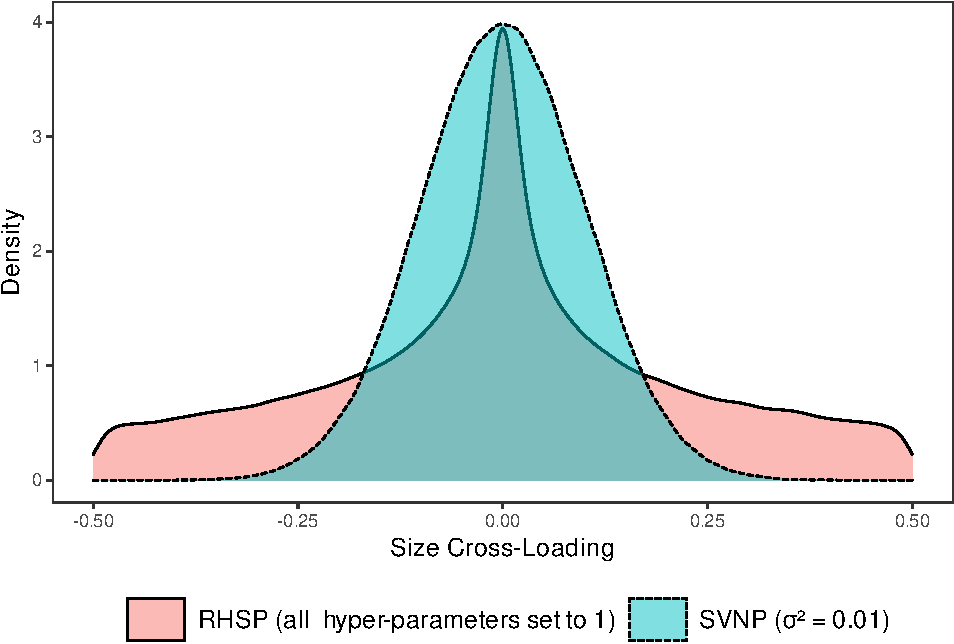
\includegraphics{JMBKoch_thesis_files/figure-latex/unnamed-chunk-1-1.pdf}
\caption{\label{fig:unnamed-chunk-1}Density Plots of the Regularization Priors of Interest.}
\end{figure}

Figure 1 compares the two shrinkage-priors that are the focus of our study. Both priors share a large peak at zero, which ensures that cross-loadings are shrunken to(wards) zero. However, the RHSP has much thicker tails. Here, for larger cross-loadings, there is thus much more prior mass than with the SVNP. This ensures large cross-loadings (and consequently other model parameters) can be estimated without bias within a single estimation step.

\hypertarget{the-current-study}{%
\section{The current study}\label{the-current-study}}

\hypertarget{study-procedure-and-parameters}{%
\subsection{Study Procedure and Parameters}\label{study-procedure-and-parameters}}

A Monte Carlo simulation study was conducted using STAN (Stan Development Team, 2021) and R (R Core Team, 2021). All code that was used to run the simulations can be openly accessed on the author's \href{https://github.com/JMBKoch/1vs2StepBayesianRegSEM}{\textbf{github}}\footnote{Specifically, the R-scripts needed to run the simulation can be found on \url{https://github.com/JMBKoch/1vs2StepBayesianRegSEM/tree/main/R}. \texttt{parameters.R} can be adjusted to adjust study parameters, and \texttt{main.R} is used to run the main simulation. Required packages are listed at the top of \texttt{parameters.R}.}. The models were sampled using the No-U-Turn-Sampler (Homan \& Gelman, 2014), with two chains, a burnin-period of 2000 and a chain-length of 4000. These sampling parameters were identified in pilot runs to be required for the RHSP to reach convergence, and were therefore also used for the SVNP in order to ensure a fair comparison.

\hypertarget{conditions}{%
\subsection{Conditions}\label{conditions}}

\hypertarget{population-conditions}{%
\subsubsection{Population Conditions}\label{population-conditions}}

The datasets were simulated based on a true 2-factor model, with three items per factor, and a factor correlation of 0.5. The true model is summarized below, both in equations (Appendix A) and graphically (Figure 2).\footnote{The stan code of the model can be found on \url{https://github.com/JMBKoch/1vs2StepBayesianRegSEM/blob/main/stan/SVNP.stan}.} The factors were scaled by fixing their means to zero and their variances to 1. All main-loadings were set to 0.75, and all residual variances to 0.3, to ensure that the largest proportion of variance in the items would be explained by their corresponding factor. We varied the size of the two truly non-zero cross-loadings \(\lambda_{c 1}\) and \(\lambda_{c 6}\) between 0.2, a negligible magnitude such that shrinkage to zero is desired, and 0.5, a size for which shrinkage towards zero should be avoided. We varied the sample sizes of the simulated datasets between 100 and 200. Larger sample sizes of for instance 500 were not included despite being common place in the literature, because adding them would have rendered the run-time of the simulations for the RHSP unfeasible. This is appropriate because for simple factor models researchers are unlikely to collect such larger sample sizes in practice.

\hypertarget{svnp-prior-conditions}{%
\subsubsection{SVNP: Prior Conditions}\label{svnp-prior-conditions}}

We varied the hyper-parameter of the SVNP, \(\sigma^2\), between 0.001, 0.01 and 0.1, based on Muthén and Asparouhov (2012). For the SVNP this left us with a total number of 2 x 2 x 3 = 12 individual sets of conditions. Per set of conditions, 200 replications were run, yielding a total of 2400 replications for this prior.

\hypertarget{rhsp-prior-conditions}{%
\subsubsection{RHSP: Prior Conditions}\label{rhsp-prior-conditions}}

The RHSP has six hyper-parameters in the specification that we apply. We varied the scales of the global shrinkage parameter \(\tau\), \(s_{global}\) between, 0.1 and 1. Here 1, is a natural maximum given that the scale generally does not become larger than 1 when applying a prior guess \(p_0\) (Piironen \& Vehtari, 2017b), and 0.1 a logical minimum given the scale of the model. Also the scale of the local shrinkage parameter \(\omega_{jk}\) was varied between, 0.1 and 1. The degrees of freedoms of these two parameters, \(df_{local}\) and \(df_{global}\) were varied between 1 and 3. For the local shrinkage parameter, larger degrees of freedoms may help to overcome sampling issues that can arise when \(df_{local} = 1\), i.e.~when the prior reduces to a half-Cauchy prior. Finally, for the scale of the distribution of \(c^2\), \(scale_{slab}\) was varied between 0.1, 1 and 5, and \(df_{slab}\) between 1 and 3. We decided to include a broader range of scales for the slab, as the slab is crucial in determining the shrinkage of large cross-loadings. We were thus left with 96 individual hyper-parameter conditions for the RHSP. In combination with the 2x2 population conditions this yielded 384 individual sets of conditions for this prior. In total there were thus \(384 \times 200 = 76800\) replications run for the RHSP.

\begin{figure}
\centering
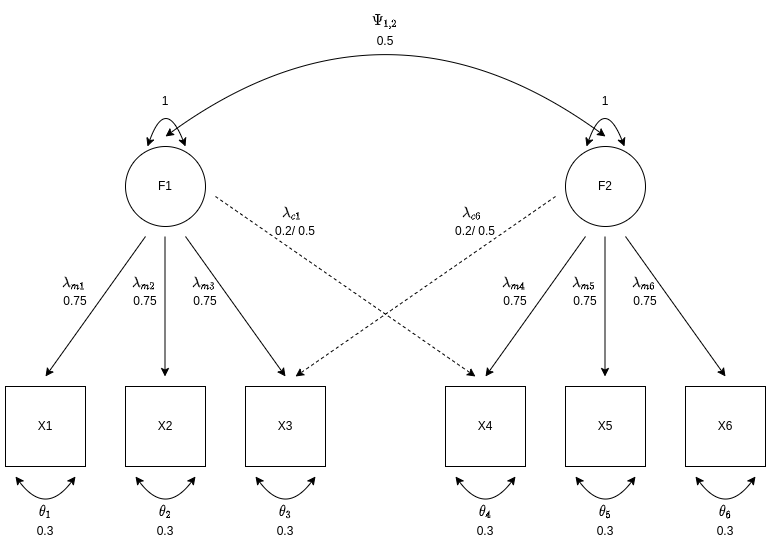
\includegraphics{~/1vs2StepBayesianRegSEM/Rmd/figures/model.png}
\caption{Graphical Representation of the True Model.}
\end{figure}

\hypertarget{outcomes}{%
\subsection{Outcomes}\label{outcomes}}

All outcomes\footnote{Summaries of all outcomes can be found on \url{https://github.com/JMBKoch/1vs2StepBayesianRegSEM/tree/main/Rmd/plots}.} were computed based on both mean and median posterior estimates of the model parameters. We only present the results of the mean estimates, but those concerning the median estimates (which do not differ relevantly from those of the mean estimates) can be accessed on github\footnote{see TBA LINK for the SVNP and TBA LINK for the RHSP}.

\hypertarget{mean-absolute-bias}{%
\subsubsection{Mean Absolute Bias}\label{mean-absolute-bias}}

For every model parameter \(\theta\) and for every set of conditions that has been sampled from for \(N_{rep}\) replications, we computed the Mean Absolute Bias:
\[\bar{Bias}_{\bar{\theta}} = \frac{1}{N_{rep}} \Sigma_{i = 1}^{N_{rep}} |\bar{\theta_i} - \theta_{true}|.\]
Given that the core issue of the SVNP is biased model estimates, this outcome naturally plays a central role in our study.

\hypertarget{relative-bias}{%
\subsubsection{Relative Bias}\label{relative-bias}}

The (Mean) Relative Bias was computed per model parameter estimate and set of conditions by dividing the estimates of the Mean Absolute Bias by the true value of the parameter:
\[\bar{Bias}_{rel, \ \bar{\theta} } = \frac{\bar{Bias}_{\bar{\theta}}}{\theta_{true} }.\]
This outcome gives an indication of the magnitude of the bias by expressing it relative to the parameter's true value. However, given the standardized scale of the true model, the Mean Absolute Bias is a quantity that can be interpreted rather intuitively in the context of this study. We therefore do not discuss these results in detail, and refer the interested reader to the study repository on github\footnote{see TBA LINK for the relative bias of the SVNP and TBA LINK for the relative bias of the RHSP}.

\hypertarget{mean-squared-error}{%
\subsubsection{Mean Squared Error:}\label{mean-squared-error}}

The Mean Squared Error (MSE) was computed per model parameter and set of conditions as:
\[MSE_{\bar{\theta}} = \frac{1}{N_{rep}} \Sigma_{i = 1}^{N_{rep}} (\bar{\theta_i} - \theta_{true})^2.\]
Another way to express the MSE is as the sum of the bias and the variance of a model parameter, which explains its added value over the Mean Absolute Bias alone. As with the Relative Bias we refrain from presenting results here as they do not add to the conclusions based on the Mean Absolute Bias\footnote{MSE estimates and plots can be found on TBA Link for the SVNP and TBA LINK for the RHSP}.

\hypertarget{power-and-type-i-error-rate}{%
\subsubsection{Power and Type-I-Error Rate}\label{power-and-type-i-error-rate}}

We computed the Mean Power (true positive rate) per set of conditions in selecting truly non-zero cross-loadings as non-zero by calculating per truly non-zero cross-loading the proportion of replications where they were selected as non-zero. The Mean Type-I-Error (false positive) rate in selecting truly zero cross-loadings as non-zero, was computed as the proportion of replications were they were selected as non-zero, per set of conditions.

For both of these outcomes, we applied a variety of selection criteria for selecting cross-loadings as non-zero, based on earlier research (Zhang et al., 2021). First, we used a variety of thresholding rules, where a cross-loading is selected as non-zero when the absolute value of its estimate exceeds a specific threshold: 0, 0.05, 0.1, 0.15. Next, we we considered four credible intervals (50\%, 80\%, 90\%, 95\%), where cross-loadings are selected as non-zero when the interval does not contain zero.

\hypertarget{results}{%
\section{Results}\label{results}}

\hypertarget{convergence}{%
\subsection{Convergence}\label{convergence}}

\hypertarget{svnp}{%
\subsubsection{SVNP}\label{svnp}}

In terms of convergence, the SVNP showed excellent performance. Across all 2400 replications there was no single parameter for which \(\hat{R} >= 1.05\). Across all parameters, the minimum value of the Effective Sample Size \(N_{eff}\) was 39.4\% of the chain length. For the largest majority of runs \(N_{eff}\) even exceeded 50\% of the chain length. Moreover, across all runs there was not a single divergent transition. All 2400 replications were therefore included in the results.

\hypertarget{rhsp}{%
\subsubsection{RHSP}\label{rhsp}}

The RHSP showed weaker performance in terms of convergence than the SVNP, although with most hyper-parameter configurations it was still acceptable, especially considering the very complex nature of the underlying model.

A total of 156 replications failed entirely, which all happend under one set of conditions: N = 100, size \(\lambda_{c1,6} = 0.2, N = 100, scale_{global} = scale_{local} = scale_{slab} = 0.1, df_{global} = df_{local} = df_{slab} = 1\). The underlying reason was likely identification issues, given the small sample sizes, and scales and degrees of freedom of the hyper-priors. We removed the remaining 44 replications of this set of conditions, as they were too little left to give a reliable picture.

Next, we removed all replications in which at least one model parameter had a value of \(\hat{R} >= 1.05\), or a value for \(N_{eff}\) smaller than 10\% of the chain-length. This removed a total of 542 replications. The maximum number of removed replications for a given set of conditions was 37, which corresponds to 18.5\% of the replications under these conditions. Below in Table 1 we present all combinations of conditions under which more than 5\% of the replications had to be removed.

\begin{table}[tbp]

\begin{center}
\begin{threeparttable}

\caption{\label{tab:unnamed-chunk-2}Conditions under which more than 5\% of replications were removed due to not reaching convergence (N = 542).}

\begin{tabular}{lllllllll}
\toprule
$scale_{global}$ & \multicolumn{1}{c}{$df_{global}$} & \multicolumn{1}{c}{$scale_{local}$} & \multicolumn{1}{c}{$df_{local}$} & \multicolumn{1}{c}{$scale_{slab}$} & \multicolumn{1}{c}{$df_{slab}$} & \multicolumn{1}{c}{N} & \multicolumn{1}{c}{Size $\lambda_{c1 , 6}$} & \multicolumn{1}{c}{N removed Rep.}\\
\midrule
0.10 & 3 & 0.10 & 1 & 0.10 & 1 & 100 & 0.50 & 10\\
0.10 & 3 & 0.10 & 1 & 1.00 & 3 & 100 & 0.50 & 11\\
0.10 & 1 & 0.10 & 1 & 5.00 & 3 & 100 & 0.50 & 12\\
0.10 & 3 & 0.10 & 1 & 5.00 & 1 & 100 & 0.50 & 12\\
0.10 & 3 & 0.10 & 1 & 1.00 & 1 & 100 & 0.50 & 13\\
0.10 & 3 & 0.10 & 3 & 0.10 & 3 & 100 & 0.50 & 13\\
0.10 & 1 & 0.10 & 1 & 5.00 & 1 & 100 & 0.50 & 15\\
0.10 & 3 & 0.10 & 1 & 5.00 & 3 & 100 & 0.50 & 15\\
0.10 & 1 & 0.10 & 3 & 0.10 & 1 & 100 & 0.50 & 20\\
0.10 & 1 & 0.10 & 3 & 1.00 & 1 & 100 & 0.50 & 24\\
0.10 & 1 & 0.10 & 3 & 1.00 & 3 & 100 & 0.50 & 24\\
0.10 & 1 & 0.10 & 3 & 5.00 & 3 & 100 & 0.50 & 27\\
0.10 & 1 & 0.10 & 3 & 5.00 & 1 & 100 & 0.50 & 30\\
0.10 & 3 & 0.10 & 3 & 0.10 & 1 & 100 & 0.50 & 33\\
0.10 & 3 & 0.10 & 3 & 1.00 & 1 & 100 & 0.50 & 34\\
0.10 & 3 & 0.10 & 3 & 5.00 & 1 & 100 & 0.50 & 34\\
0.10 & 3 & 0.10 & 3 & 1.00 & 3 & 100 & 0.50 & 37\\
0.10 & 3 & 0.10 & 3 & 5.00 & 3 & 100 & 0.50 & 37\\
\bottomrule
\addlinespace
\end{tabular}

\begin{tablenotes}[para]
\normalsize{\textit{Note.} Replications were removed for having an $\hat{R} >= 1.05$ or an $N_{eff}$  smaller that 10\% of the chain-length, for any of the model parameters.}
\end{tablenotes}

\end{threeparttable}
\end{center}

\end{table}

Table 2 presents all sets of conditions under which there were, on average, at least 5\% divergent transitions per chain. We decided not to remove these replications, as this would have removed a substantial number of 4474 replications. In general, it is advised not to include any divergent transitions, since they introduce bias. Given the complex nature of the RHSP, which in practice usually leads to some divergent transitions, it is hard to follow this advise in practice. However, it needs to be taken into account in the interpretation of the findings that the divergent transitions may have added bias to the model estimates of the RHSP.

\begin{table}[tbp]

\begin{center}
\begin{threeparttable}

\caption{\label{tab:unnamed-chunk-3}Conditions with on average more than 5\% divergent transitions.}

\begin{tabular}{lllllllll}
\toprule
$scale_{global}$ & \multicolumn{1}{c}{$df_{global}$} & \multicolumn{1}{c}{$scale_{local}$} & \multicolumn{1}{c}{$df_{local}$} & \multicolumn{1}{c}{$scale_{slab}$} & \multicolumn{1}{c}{$df_{slab}$} & \multicolumn{1}{c}{N} & \multicolumn{1}{c}{Size $\lambda_{c1 , 6}$} & \multicolumn{1}{c}{Mean Prop. Div.}\\
\midrule
0.10 & 1 & 0.10 & 3 & 0.10 & 1 & 100 & 0.50 & 0.09\\
0.10 & 1 & 0.10 & 3 & 1.00 & 1 & 100 & 0.50 & 0.08\\
0.10 & 1 & 0.10 & 3 & 5.00 & 1 & 100 & 0.50 & 0.08\\
0.10 & 1 & 0.10 & 3 & 5.00 & 3 & 100 & 0.50 & 0.08\\
0.10 & 3 & 0.10 & 1 & 0.10 & 1 & 100 & 0.50 & 0.10\\
0.10 & 3 & 0.10 & 1 & 1.00 & 1 & 100 & 0.50 & 0.08\\
0.10 & 3 & 0.10 & 1 & 5.00 & 1 & 100 & 0.50 & 0.09\\
0.10 & 3 & 0.10 & 1 & 5.00 & 3 & 100 & 0.50 & 0.08\\
0.10 & 3 & 0.10 & 3 & 0.10 & 1 & 100 & 0.50 & 0.10\\
0.10 & 3 & 0.10 & 3 & 1.00 & 1 & 100 & 0.50 & 0.11\\
0.10 & 3 & 0.10 & 3 & 1.00 & 3 & 100 & 0.50 & 0.07\\
0.10 & 3 & 0.10 & 3 & 5.00 & 1 & 100 & 0.50 & 0.11\\
0.10 & 3 & 0.10 & 3 & 5.00 & 3 & 100 & 0.50 & 0.12\\
\bottomrule
\addlinespace
\end{tabular}

\begin{tablenotes}[para]
\normalsize{\textit{Note.} There was a total of 4474 replications were the divergent transitions exceeded 5\% of the chain-length. There were 19036 replications with more than 1\% of divergent transitions. There were 1970 replications with more than 10\% of divergent transitions. There were 186 replications with more than 50\% of divergent transitions.}
\end{tablenotes}

\end{threeparttable}
\end{center}

\end{table}

\hypertarget{main-results}{%
\subsection{Main Results}\label{main-results}}

\hypertarget{mean-absolute-bias-svnp}{%
\subsubsection{Mean Absolute Bias: SVNP}\label{mean-absolute-bias-svnp}}

The Mean Absolute Bias of the SVNP for all parameters is summarized in Figure 3. For parameter estimates that show an identical pattern (\(\bar{\lambda}_{c 2-5}\), \(\bar{\lambda}_{c 1, 6}\), \(\bar{\lambda}_{m 1, 2, 5, 6}\), \(\bar{\lambda}_{m 3-4}\), and \(\bar{\theta}_{1-6}\)), the first respecting estimate is presented representative for all, both in Figure 3 and in the numbers presented below. As results are almost identical for the two sample sizes, we focus on presenting the findings for N = 100, to not distract from our main conclusions.\footnote{The Mean Absolute Bias of the SVNP visualized for the different sample sizes separately can be found on \url{https://github.com/JMBKoch/1vs2StepBayesianRegSEM/blob/main/Rmd/plots/plotsBiasSVNP.html}.}

\begin{figure}
\centering
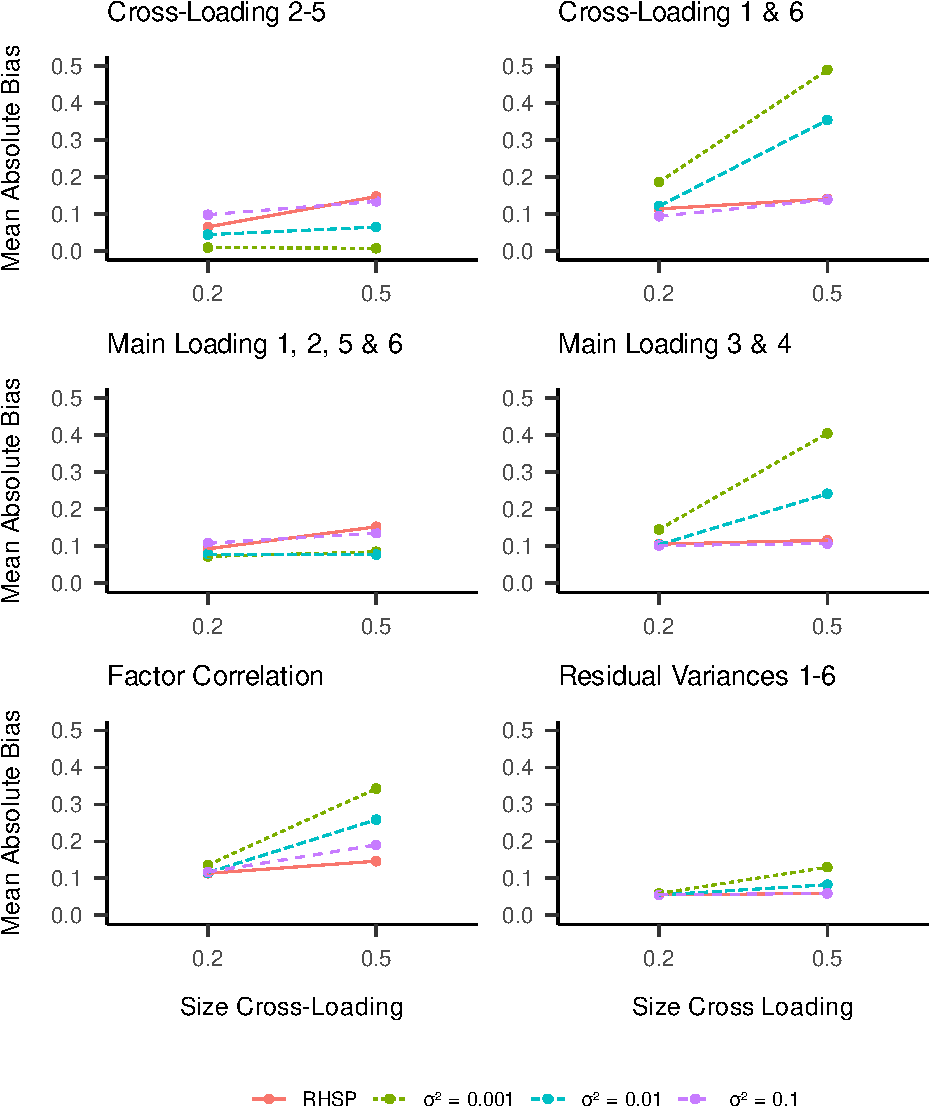
\includegraphics{JMBKoch_thesis_files/figure-latex/unnamed-chunk-4-1.pdf}
\caption{\label{fig:unnamed-chunk-4}Mean Absolute Bias in the Model Parameters (N = 100). Per set of parameters that showed an identical pattern, the first parameter was used to represent all other parameters, e.g.~cross-loading 2 was plottet representative for cross-loading 1 and 3-5. All hyperparameters of the RHSP are set to 1 in the results presented here.}
\end{figure}

Figure 3 shows that, as expected, there was substantial bias in some parameter estimates. While the bias in the posterior means of the truly zero cross-loadings \(\bar{\lambda}_{c 2-5}\) was relatively small, it was pronounced in the estimates of the truly non-zero cross-loadings \(\bar{\lambda}_{c 1}\) and \(\bar{\lambda}_{c 6}\). Particularly with a large true cross-loading of 0.5 and \(\sigma^2 = 0.001\) the bias was very large, e.g.~\(\bar{Bias}_{\bar{\lambda}_{c 1}} = 0.49\), since the estimates of the true cross-loadings of 0.5 were shrunken almost entirely to zero (e.g.~\(\bar{\lambda}_{c 1} = 0.01\)). The choice of \(\sigma^2\) played a crucial role here. Also with \(\sigma^2 = 0.01\) (and true cross-loadings of 0.5) substantial bias occured (e.g.~\(\bar{Bias}_{\bar{\lambda}_{c 1}} = 0.35\)), as the cross-loading were still under-estimated considerably (\(\bar{\lambda}_{c 1} = 0.15\)), though not entirely shrunken to zero. With \(\sigma^2 = 0.1\) the bias in the estimates of the cross-loadings was less pronounced (e.g.~\(\bar{Bias}_{\bar{\lambda}_{c 1}} = 0.14\)). Here \(\sigma^2\) was large enough to estimate the cross-loadings closer to their true value, \(\bar{\lambda}_{c 1} = 0.37\).

Also the estimates of the main loadings of factor 1 on item 3 (\(\bar{\lambda}_{m 3}\)) and of factor 2 on item 4 (\(\bar{\lambda}_{m 4}\)) were substantially biased when the true cross-loadings were 0.5 and \(\sigma^2 = 0.001\) (e.g.~\(\bar{Bias}_{\bar{\lambda}_{m 3}} = 0.40\)). These two loadings showed much higher bias than the other four main-loadings as they loaded on the same two items as the two non-zero cross-loadings (\(\bar{\lambda}_{c 1}\) and \(\bar{\lambda}_{c 6}\), see Figure 2). As the cross-loadings were shrunken to zero, these main loadings now also had to account for the variance in the items that was truly explained by the cross-loadings. Consequently, the two main-loadings were over-estimated, e.g.~\(\bar{\lambda}_{m 3} = 1.15\).

In the factor correlation the bias was also relatively small and approximately the same for the different values of \(\sigma^2\) when the truly non-zero cross-loadings were 0.2. Again, bias became much more pronounced with true cross-loadings of 0.5, especially when \(\sigma^2 = 0.001\) (\(\bar{Bias}_{\bar{\Psi}_{1,2}} = 0.34\)). In this situation the factor correlation was heavily over-estimated (\(\bar{\Psi}_{1,2} = 0.84\)). This was because the covariance between item 3 and 4 that arose from the two cross-loadings, was mis-attributed to the factor-correlation, as the cross-loadings were shrunken to zero.

The bias in the estimates of the residual variances \(\bar{\theta}_{1-6}\) was not large across different conditions, although also here a noticeable increase occurs between true cross-loadings of 0.2 and 0.5 when \(\sigma^2 = 0.001\).

\hypertarget{mean-absolute-bias-rhsp}{%
\subsubsection{Mean Absolute Bias: RHSP}\label{mean-absolute-bias-rhsp}}

Figure 3 illustrates the Mean Absolute Bias of the RHSP for N = 100 and all hyper-parameters of the RHSP set to one. Again, since patterns were identical across sets of parameters, the first respecting parameter per set is reported representative for the whole set. We extensively compared the Mean Absolute Bias of the RHSP between different hyper-parameter settings and sample sizes\footnote{see \url{https://github.com/JMBKoch/1vs2StepBayesianRegSEM/blob/main/Rmd/analyses/RHSP/plotsBiasRHSP.html}}. Differences were so little that we do not present them here, to not distract from our main comparison to the SVNP. We decided to present the findings with all hyper-parameters set to one, as this is a logical default hyper-parameter configuration under the scale of a standardized CFA model. The replications under these conditions showed good convergence, such that only a single replication had to be removed.

In general, the RHSP showed very similar patterns to the SVNP with \(\sigma^2 = 0.1\), and therefore substantially less bias than the SVNP under most hyper-parameter settings. For estimates of the truly zero cross-loadings \(\bar{\lambda}_{c 2-5}\), the bias was relatively little, although here it was actually slightly larger than for the SVNP with \(\sigma^2 = 0.1\). Note that the bias in these cross-loadings comes from these cross-loading, on average, being under-estimated, for instance under cross-loadings of 0.5 (\(\bar{\lambda}_{c, 2} = -0.14\)).

For estimates of the truly non-zero cross-loadings \(\bar{\lambda}_{c1,6}\), the bias was lower than for the SVNP with \(\sigma^2 = 0.01\), or \(\sigma^2 = 0.01\) when the true cross-loadings were 0.2. Most importantly, under true cross-loadings of 0.5, bias was substantially lower than that of the SVNP with \(\sigma^2 = 0.01, \ 0.01\) (e.g.~\(\bar{Bias}_{\bar{\lambda}_{c 1}} = 0.14\)). Here, the the RHSP allowed the large cross-loadings to mostly escape the shrinkage (\(bar{\lambda}_{c 1}\) = 0.37), although there was still some shrinkage present.

Also with regard to main-loadings the RHSP performed strikingly similar to the SVNP with \(\sigma^2 = 0.1\). In general, the bias was thus lower than for the SVNP under most hyper-parameter settings. Especially for \(\lambda_{m,3-4}\) and under true cross-loadings of 0.5 the differences between the RHSP and the SVNP with \(\sigma^2 = 0.01, \ 0.01\) were substantial.

For the factor correlation, the RHSP had the least amount of bias, with true cross-loadings of 0.5 (\(\bar{Bias}_{\bar{\Psi}_{1,2}}\) = 0.15) almost being indistinguishable form the bias with cross-loadings of 0.2 (\(\bar{Bias}_{\bar{\Psi}_{1,2}}\) = 0.11). The factor correlation was slightly over-estimated, for instance under true cross-loadings of 0.5 \(\bar{\Psi}_{1,2} = 0.64\).

Also regarding the bias in the estimates of the residual variances \(\bar{\theta}_{1-6}\), the pattern of the RHSP was indistinguishable from that of the SVNP with \(\sigma^2 = 0.1\).

~

\hypertarget{power-and-type-i-error-rate-svnp}{%
\subsubsection{Power and Type-I-Error Rate: SVNP}\label{power-and-type-i-error-rate-svnp}}

\begin{figure}
\centering
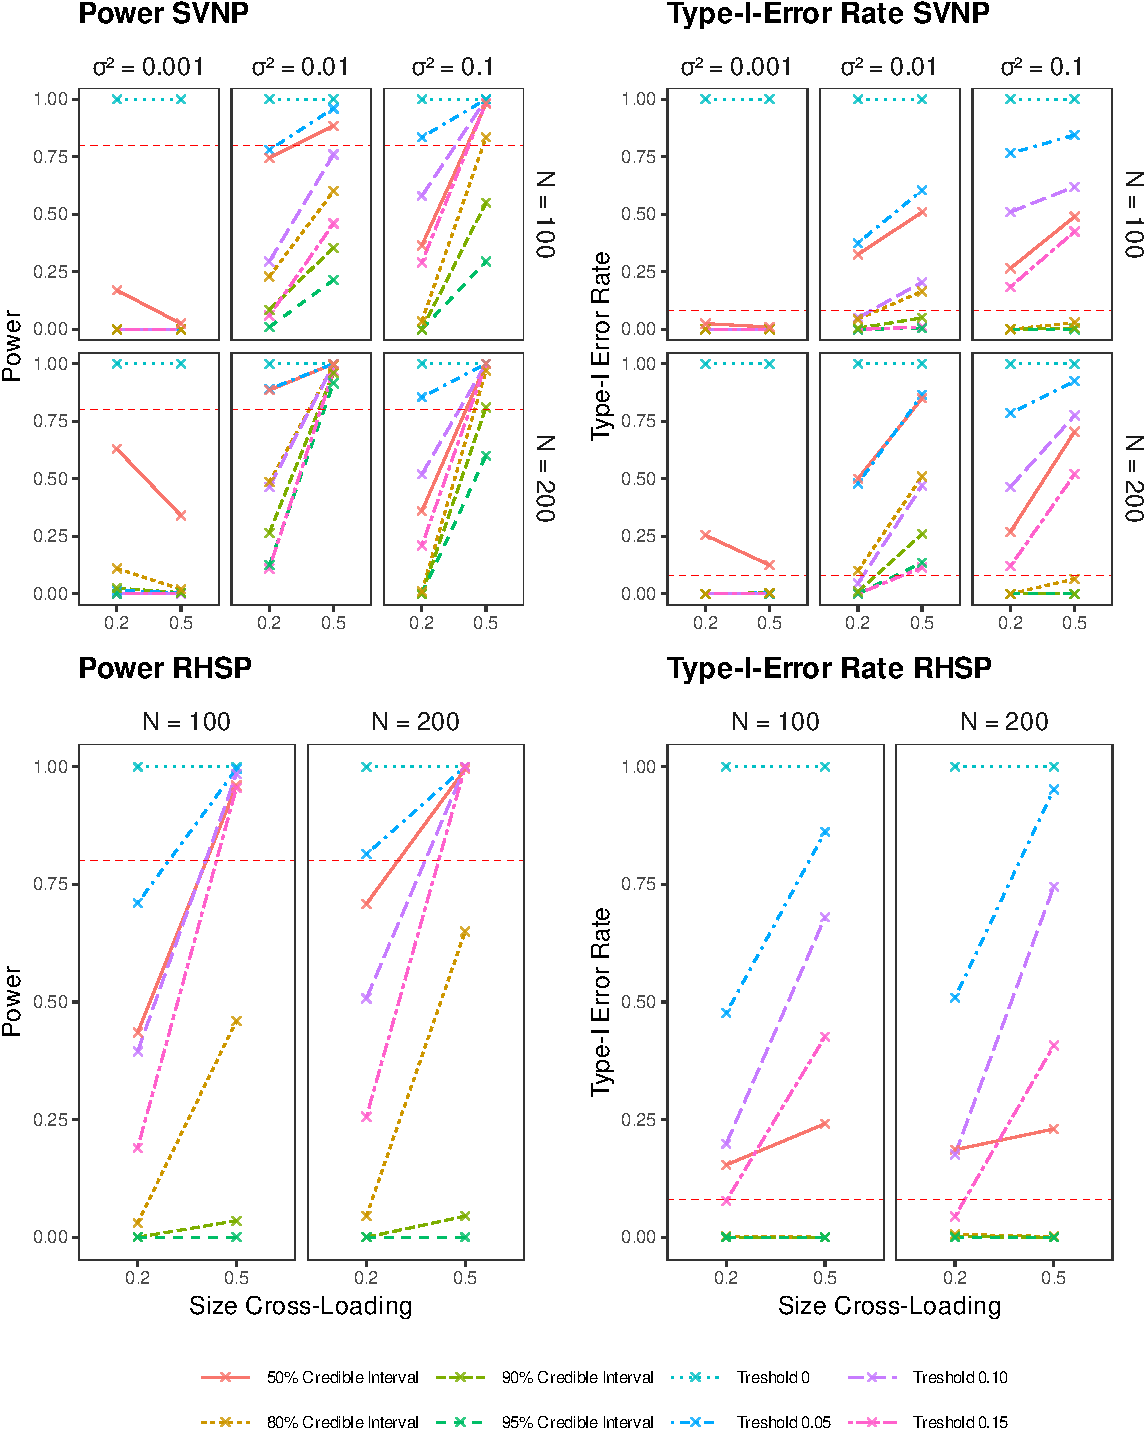
\includegraphics{JMBKoch_thesis_files/figure-latex/unnamed-chunk-5-1.pdf}
\caption{\label{fig:unnamed-chunk-5}Mean Power and Type-I-Error Rates in Selecting non-zero Crossloadings. All hyper-parameters of the RHSP are set to 1 in the results presented here.}
\end{figure}

The top left panel of Figure 4 summarizes the Power (true-positive rate) in selecting the truly non-zero cross-loadings as non-zero of the SVNP, per set of conditions and selection criterion. Again, the outcomes are presented for the first parameter of an identical set of parameters (i.e., \(\lambda_{c,1}\) is presented representative for the two truly non-zero cross-loadings). The horizontal red dash line indicates the minimum power of .80 recommended by Muthén and Asparouhov (2012).

With a threshold of 0.00 there is a perfect power of 1 in selecting non-zero cross loadings. This is logical, since in Bayesian inference posterior means will never be entirely zero (Zhang et al., 2021). The result thus mostly serves to illustrate this property of Bayesian inference and thereby the need for more complex selection rules in Bayesian regularization, if the goal is variable selection itself, and not only unbiased model parameter estimates.

Next, we can see that across most conditions, the Power falls under the desired threshold of 0.8. When \(\sigma^2 = 0.001\) non-zero cross-loadings were always over-shrunken so much that they were never selected as non-zero. Under \(\sigma^2 = 0.01\), the situation improved somewhat, with now cross-loadings of 0.5 being correctly selected as non zero for all selecting rules when N = 200. For N = 100, thresholds of 0.05, and 50\% credible intervals also had the desired levels of power, with thresholds of 0.10 also almost reaching a power of .80. The SVNP performed best in terms of power when \(\sigma^2 = 0.1\). With N = 200, all selection rules except for the 95\% credible intervals reached the desired Power. With N = 100, all selection rules except for the 95\% and 90\% credible intervals exceeded a power of 0.80.

The top right panel of Figure 4 summarizes the Mean Type-I-Error rate of the SVNP. According to Cham, West, Ma, and Aiken (2012), the maximally acceptable Type-I-Error rate is the upper-bound of a 95\% interval of a binomial distribution, in this case \(0.05 + 1.96 \times \sqrt{0.05 \times (1-0.05)/ N_{rep}} = 0.08\). As with the Power, there is a Type-I-Error rate of 1 with the tresholding rule of 0.00, as posterior means are never entirely zero. In general, under most configurations the Type-I-Error rate exceeded the desired maximum. Under \(\sigma^2 = 0.001\) and N = 100, the Type-I-Error rate stayed very low, as under this condition all cross-loadings, including the truly zero ones, were always shunken almost entirely to zero, such that only a treshold of 0.00 would lead to selecting them as non-zero. With N = 200, also the 50\% credible intervals lead to an undesiredly large Type-I error rate. With \(\sigma^2 = 0.01\) and N = 100, some selection rules (90\% \& 95\% credible intervals, a treshold of 0.15) had an acceptable Type-I-Error rate even with large true cross-loadings of 0.5. Most selection rules, however, exceeded a Type-I-Error rate of 0.8, especially under true non-zero cross-loadings of 0.5. With \(\sigma^2 = 0.1\), all selection rules except for 90\% and 95\% credible intervals had unacceptably high Type-I-Error rates for both sizes of non-zero cross-loadings, even though pronounced differences between cross-loadings of 0.2 and 0.5 existed. This is explained by the fact that cross-loadings were mostly estimated as lower than zero under this set of conditions.

\hypertarget{power-and-type-i-error-rate-rhsp}{%
\subsubsection{Power and Type-I-Error Rate: RHSP}\label{power-and-type-i-error-rate-rhsp}}

For the RHSP, the overall power an Type-I-Error rate also did not live up to the standards by Muthén and Asparouhov (2012) and Cham et al. (2012). As with the SVNP, the tresholding rule with a threshold of 0.00 lead to both a perfect power and Type-I-Error rate.

The bottom left panel of Figure 4 shows the Power in selecting the first truly non-zero cross-loading (\(\lambda_{c,1}\)) of the RHSP with all hyper-parameters set to 1.The desired power was exclusively reached in selecting cross-loadings that were truly 0.5. This only happened for 50\% credible intervals, and the three tresholds. Especially the widest (90\% and 95\%) credible intervals performed very poorly, which is explained by the fact that the lower bounds of these intervals (almost) always exceeded zero.

The bottom right panel of Figure 4 shows the Type-I-Error in wrongly selecting the first truly zero cross-loading (\(\lambda_{c,2}\)) as nonzero of the RHSP with all hyper-parameters set to 1. Only the 90\% and 95\% stayed within the desired boundary, as they always included zero.

\hypertarget{conclusions-and-discussion}{%
\section{Conclusions and Discussion}\label{conclusions-and-discussion}}

This was the first study to apply the Regularized Horseshoe Prior (RHSP, Piironen \& Vehtari, 2017b) in Bayesian Regularized SEM, by using it to select cross-loadings in CFA. A comparison to the classic Bayesian CFA approach by Muthén and Asparouhov (2012), where cross-loadings are regularized throughwith the SVNP, was made. It was found that, as expected, generally the RHSP was able to estimate the model parameters of a CFA model with substantially less bias than the SVNP.

The SVNP performed well under small true non-zero cross-loadings in terms of estimating the model without substantial bias. This can be interpreted as a successful instance of regularization, where an acceptable amount of bias is added to the model by shrinking some parameters to zero, to reach a more sparse solution. However, with larger truly non-zero cross-loadings, the performance of the SVNP decreased substantially. With smaller values of \(\sigma^2\), particularly with \(\sigma^2 = 0.001\), these cross-loadings were still shrunken to zero, even though they were much larger in reality. This caused substantial bias, not only in the estimates of the cross-loadings itself, but also in the estimates of some main-loadings and the factor correlation. In practice, bias in structural parameters is particularly concerning, as it may lead to wrong conclusions in research on structural relationships between latent constructs.

In contrast, the RHSP was able to estimate the model with relatively little bias, even with larger cross-loadings and across different sample sizes. This indicates that the desired property of the RHSP of letting large parameters escape shrinkage also applies to cross-loadings in CFA. Hereby, the RHSP proved to be robust to different sample sizes and hyper-parameter configurations. With \(\sigma^2 = 0.1\), the SVNP actually had almost identically low levels of bias as the RHSP.Such relatively large variance still allowed for enough deviations from zero in the cross-loadings to yield relatively accurate estimates of the non-zero cross-loadings itself and consequently the other model parameters. Hence, under this configuration, the SVNP performed as well as the RHSP. However, we are convinced that simply using larger values of \(\sigma^2\) with the SVNP is no general alternative to the RHSP. In practice, models may include more structural parameters, even more cross-loadings, or a number of residual co-variances. Under these circumstances, large values of \(\sigma^2\) may lead to identification issues. Moreover, the larger \(\sigma^2\), the more cross-loadings will be selected as non-zero, which may ultimately lead to over-fitting. Nevertheless, under simple models such as the one employed in this study using the less complex SVNP may prove advantageous in practice. Not only does the SVNP take substantially less time to sample and has better performance in terms of convergence than the RHSP, it also does not risk bias in the estimated due to rows removed because of non-convergence, or because of divergent transitions (Although note that we were not able to directly identify bias through divergent transitions). Under more complex models the RHSP is more advisable, although future research comparing the SVNP to the RHSP in regularizing more complex SEM-models is yet to illustrate this directly.

Regarding the Power and Type-I-Error rate in selecting cross-loadings as non-zero, both priors performed poorly across a range of selection rules. First of all, this is not surprising, given earlier research which clearly showed that a range of shrinkage priors (SVNP, Bayesian LASSOO, Spike-and-Slab Prior, Lu et al., 2016; Zhang et al., 2021) generally need much larger sample sizes than the one's employed in this study to reach desirable levels of Power and Type-I-Error rates (see also Jacobucci et al., 2016; Lu et al., 2016, who show that also frequentist variable selection methods are very sensitive to sample size). Future research should therefore assess the Power and Type-I-Error rate of the RHSP under larger sample sizes (e.g.~N = 500, 1000, 2000) to allow for a more conclusive picture. Note, however, that our findings do not imply that the RHSP is useless under low sample sizes. If the goal of regularization is not to select which cross-loadings are zero, but to yield unbiased estimates of the other model parameters, the RHSP still works better than the SVNP under most settings, even with small sample sizes. In practice, researchers often fit SEM-models including a measurement structure to test structural hypotheses. For this purpose, the question of whether or not cross-loadings are zero is not relevant, as long as the structural model parameters are estimated without substantial bias. In general, the large levels of bias found in the SVNP are not surprising, given the original approach explicitly asks for a 2-step approach (Muthén \& Asparouhov, 2012). However, the fact that the SVNP performed so poorly in selecting the cross-loadings suggests that in practice the 2-step approach, which heavily relies on a correct selection of cross-loadings as non-zero, is not advisable.

Next to specific limitations named above, the current study has some general shortcomings, which lead to a number of recommendations for future research. First, we only assessed the performance of the RHSP in regularizing cross-loadings in a very simple CFA model consisting of only two factors. A straightforward way of extending the current study and making its findings more generalizable would be to also include factor models with more factors in future research. Within simple CFA models, another important set of parameters that can be identified through the usage of shrinkage-priors are residual co-variances (i.e.~the off-diagonal elements of \(\Theta\)), which are also usually fixed to zero in classic CFA (Muthén \& Asparouhov, 2012). An important next step is thus to assess the performance of the RHSP in selecting residual co-variances on top of cross-loadings. Of course, it is also desirable to assess the performance of the RHSP in regularizing model-parameters in more complex SEM models, such as structural parameters, e.g.~indirect effects in mediation models, or regression coefficients in MIMIC models. Also applying the RHSP in measurement models with non-continuous (i.e., binary, ordinal or nominal) outcomes would be an interesting way of building on the current study. Next to these directions for future research, the promising findings for the RHSP in Bayesian CFA call for an implementation of the RSHP into standard Bayesian SEM software (e.g.~by adding it to the BLAVAAN package, Merkle, Fitzsimmons, Uanhoro, \& Goodrich, 2020), such that applied researchers can actually take advantage of it in practice.

Despite the limitations names, the current study formed a valuable contribution to the current literature. We showed that the RHSP can successfully be applied in Bayesian CFA and our findings point to both a number of fruitful avenues of future research as well as a numer of general implications for implementing the RHSP in practice .

\clearpage

\hypertarget{references}{%
\section{References}\label{references}}

\begingroup
\setlength{\parindent}{-0.5in}
\setlength{\leftskip}{0.5in}

\hypertarget{refs}{}
\begin{CSLReferences}{1}{0}
\leavevmode\vadjust pre{\hypertarget{ref-betancourt_conceptual_2018}{}}%
Betancourt, M. (2018). A {Conceptual} {Introduction} to {Hamiltonian} {Monte} {Carlo}. \emph{arXiv:1701.02434 {[}Stat{]}}. Retrieved from \url{http://arxiv.org/abs/1701.02434}

\leavevmode\vadjust pre{\hypertarget{ref-bollen_structural_1989}{}}%
Bollen, K. A. (1989). \emph{Structural {Equations} with {Latent} {Variables}}. John Wiley \& Sons.

\leavevmode\vadjust pre{\hypertarget{ref-carvalho_horseshoe_2010}{}}%
Carvalho, C. M., Polson, N. G., \& Scott, J. G. (2010). The horseshoe estimator for sparse signals. \emph{Biometrika}, \emph{97}(2), 465--480. \url{https://doi.org/10.1093/biomet/asq017}

\leavevmode\vadjust pre{\hypertarget{ref-cham_estimating_2012}{}}%
Cham, H., West, S. G., Ma, Y., \& Aiken, L. S. (2012). Estimating {Latent} {Variable} {Interactions} {With} {Nonnormal} {Observed} {Data}: {A} {Comparison} of {Four} {Approaches}. \emph{Multivariate Behavioral Research}, \emph{47}(6), 840--876. \url{https://doi.org/10.1080/00273171.2012.732901}

\leavevmode\vadjust pre{\hypertarget{ref-chen_jinsong_partially_2021}{}}%
Chen, J., Guo, Zhihan, Zhang, Lijin, \& Pan, Junhao. (2021). A {Partially} {Confirmatory} {Approach} to {Scale} {Development} {With} the {Bayesian} {Lasso}. \emph{Psychological Methods}, \emph{26}(2), 210--235. Retrieved from \url{https://oce-ovid-com.proxy.library.uu.nl/article/00060744-202104000-00005/HTML}

\leavevmode\vadjust pre{\hypertarget{ref-cox_principles_2006}{}}%
Cox, D. R. (2006). \emph{Principles of {Statistical} {Inference}}. Cambridge University Press.

\leavevmode\vadjust pre{\hypertarget{ref-datta_asymptotic_2013}{}}%
Datta, J., \& Ghosh, J. K. (2013). Asymptotic properties of {Bayes} risk for the horseshoe prior. \emph{Bayesian Analysis}, \emph{8}(1), 111--132.

\leavevmode\vadjust pre{\hypertarget{ref-george_variable_1993}{}}%
George, E. I., \& McCulloch, R. E. (1993). Variable {Selection} {Via} {Gibbs} {Sampling}. \emph{Journal of the American Statistical Association}, \emph{88}(423), 881--889. \url{https://doi.org/10.2307/2290777}

\leavevmode\vadjust pre{\hypertarget{ref-ghosh_use_2018}{}}%
Ghosh, J., Li, Y., \& Mitra, R. (2018). On the {Use} of {Cauchy} {Prior} {Distributions} for {Bayesian} {Logistic} {Regression}. \emph{Bayesian Analysis}, \emph{13}(2), 359--383. \url{https://doi.org/10.1214/17-BA1051}

\leavevmode\vadjust pre{\hypertarget{ref-guo_bayesian_2012}{}}%
Guo, R., Zhu, H., Chow, S.-M., \& Ibrahim, J. G. (2012). Bayesian {Lasso} for {Semiparametric} {Structural} {Equation} {Models}. \emph{Biometrics}, \emph{68}(2), 567--577. \url{https://doi.org/10.1111/j.1541-0420.2012.01751.x}

\leavevmode\vadjust pre{\hypertarget{ref-hans_bayesian_2009}{}}%
HANS, C. (2009). Bayesian lasso regression. \emph{Biometrika}, \emph{96}(4), 835--845. Retrieved from \url{https://www.jstor.org/stable/27798870}

\leavevmode\vadjust pre{\hypertarget{ref-hastie_statistical_2015}{}}%
Hastie, T., Tibshirani, R., \& Wainwright, M. (2015). Statistical learning with sparsity. \emph{Monographs on Statistics and Applied Probability}, \emph{143}, 143.

\leavevmode\vadjust pre{\hypertarget{ref-hoerl_ridge_2000}{}}%
Hoerl, A. E., \& Kennard, R. W. (2000). Ridge {Regression}: {Biased} {Estimation} for {Nonorthogonal} {Problems}. \emph{Technometrics}, \emph{42}(1), 80--86. \url{https://doi.org/10.2307/1271436}

\leavevmode\vadjust pre{\hypertarget{ref-homan_no-u-turn_2014}{}}%
Homan, M. D., \& Gelman, A. (2014). The {No}-{U}-turn sampler: Adaptively setting path lengths in {Hamiltonian} {Monte} {Carlo}. \emph{The Journal of Machine Learning Research}, \emph{15}(1), 1593--1623.

\leavevmode\vadjust pre{\hypertarget{ref-hsiang_bayesian_1975}{}}%
Hsiang, T. C. (1975). A {Bayesian} {View} on {Ridge} {Regression}. \emph{Journal of the Royal Statistical Society. Series D (The Statistician)}, \emph{24}(4), 267--268. \url{https://doi.org/10.2307/2987923}

\leavevmode\vadjust pre{\hypertarget{ref-ishwaran_spike_2005}{}}%
Ishwaran, H., \& Rao, J. S. (2005). Spike and slab variable selection: {Frequentist} and {Bayesian} strategies. \emph{The Annals of Statistics}, \emph{33}(2), 730--773. \url{https://doi.org/10.1214/009053604000001147}

\leavevmode\vadjust pre{\hypertarget{ref-jacobucci_practical_2019}{}}%
Jacobucci, R., Brandmaier, A. M., \& Kievit, R. A. (2019). A {Practical} {Guide} to {Variable} {Selection} in {Structural} {Equation} {Modeling} by {Using} {Regularized} {Multiple}-{Indicators}, {Multiple}-{Causes} {Models}. \emph{Advances in Methods and Practices in Psychological Science}, \emph{2}(1), 55--76. \url{https://doi.org/10.1177/2515245919826527}

\leavevmode\vadjust pre{\hypertarget{ref-jacobucci_comparison_2018}{}}%
Jacobucci, R., \& Grimm, K. J. (2018). Comparison of {Frequentist} and {Bayesian} {Regularization} in {Structural} {Equation} {Modeling}. \emph{Structural Equation Modeling: A Multidisciplinary Journal}, \emph{25}(4), 639--649. \url{https://doi.org/10.1080/10705511.2017.1410822}

\leavevmode\vadjust pre{\hypertarget{ref-jacobucci_regularized_2016}{}}%
Jacobucci, R., Grimm, K. J., \& McArdle, J. J. (2016). Regularized {Structural} {Equation} {Modeling}. \emph{Structural Equation Modeling: A Multidisciplinary Journal}, \emph{23}(4), 555--566. \url{https://doi.org/10.1080/10705511.2016.1154793}

\leavevmode\vadjust pre{\hypertarget{ref-james_introduction_2021}{}}%
James, G., Witten, D., Hastie, T., \& Tibshirani, R. (2021). \emph{An {Introduction} to {Statistical} {Learning}: With {Applications} in {R}}. New York, NY: Springer US. \url{https://doi.org/10.1007/978-1-0716-1418-1}

\leavevmode\vadjust pre{\hypertarget{ref-lu_bayesian_2016}{}}%
Lu, Z.-H., Chow, S.-M., \& Loken, E. (2016). Bayesian {Factor} {Analysis} as a {Variable}-{Selection} {Problem}: {Alternative} {Priors} and {Consequences}. \emph{Multivariate Behavioral Research}, \emph{51}(4), 519--539. \url{https://doi.org/10.1080/00273171.2016.1168279}

\leavevmode\vadjust pre{\hypertarget{ref-maccallum_model_1992}{}}%
MacCallum, R. C., Roznowski, M., \& Necowitz, L. B. (1992). Model modifications in covariance structure analysis: The problem of capitalization on chance. \emph{Psychological Bulletin}, \emph{111}(3), 490--504. \url{https://doi.org/10.1037/0033-2909.111.3.490}

\leavevmode\vadjust pre{\hypertarget{ref-merkle_efficient_2020}{}}%
Merkle, E. C., Fitzsimmons, E., Uanhoro, J., \& Goodrich, B. (2020). Efficient {Bayesian} {Structural} {Equation} {Modeling} in {Stan}. \emph{arXiv:2008.07733 {[}Stat{]}}. Retrieved from \url{http://arxiv.org/abs/2008.07733}

\leavevmode\vadjust pre{\hypertarget{ref-mitchell_bayesian_1988}{}}%
Mitchell, T. J., \& Beauchamp, J. J. (1988). Bayesian {Variable} {Selection} in {Linear} {Regression}. \emph{Journal of the American Statistical Association}, \emph{83}(404), 1023--1032. \url{https://doi.org/10.2307/2290129}

\leavevmode\vadjust pre{\hypertarget{ref-muthen_bsem_2013}{}}%
Muthen, B., \& Asparouhov, T. (2013). {BSEM} {Measurement} {Invariance} {Analysis}. \emph{Mplus Webntoes}. Retrieved from \url{https://www.statmodel.com/examples/webnotes/webnote17.pdf}

\leavevmode\vadjust pre{\hypertarget{ref-muthen_bayesian_2012}{}}%
Muthén, B., \& Asparouhov, T. (2012). Bayesian {SEM}: {A} more flexible representation of substantive theory, 78. \url{https://doi.org/10.1037/a0026802}

\leavevmode\vadjust pre{\hypertarget{ref-park_bayesian_2008}{}}%
Park, T., \& Casella, G. (2008). The {Bayesian} {Lasso}. \emph{Journal of the American Statistical Association}, \emph{103}(482), 681--686. \url{https://doi.org/10.1198/016214508000000337}

\leavevmode\vadjust pre{\hypertarget{ref-piironen_hyperprior_2017}{}}%
Piironen, J., \& Vehtari, A. (2017a). On the {Hyperprior} {Choice} for the {Global} {Shrinkage} {Parameter} in the {Horseshoe} {Prior}. In \emph{Proceedings of the 20th {International} {Conference} on {Artificial} {Intelligence} and {Statistics}} (pp. 905--913). PMLR. Retrieved from \url{https://proceedings.mlr.press/v54/piironen17a.html}

\leavevmode\vadjust pre{\hypertarget{ref-piironen_sparsity_2017}{}}%
Piironen, J., \& Vehtari, A. (2017b). Sparsity information and regularization in the horseshoe and other shrinkage priors. \emph{Electronic Journal of Statistics}, \emph{11}(2), 5018--5051. \url{https://doi.org/10.1214/17-EJS1337SI}

\leavevmode\vadjust pre{\hypertarget{ref-polson_shrink_2010}{}}%
Polson, N. G., \& Scott, J. G. (2010). Shrink globally, act locally: {Sparse} {Bayesian} regularization and prediction. \emph{Bayesian Statistics}, \emph{9}(501-538), 105.

\leavevmode\vadjust pre{\hypertarget{ref-r_core_team_r_2021}{}}%
R Core Team. (2021). R: {A} {Language} and {Environment} for {Statistical} {Computing}. Retrieved from \url{https://www.R-project.org/}

\leavevmode\vadjust pre{\hypertarget{ref-serang_exploratory_2020}{}}%
Serang, S., \& Jacobucci, R. (2020). Exploratory {Mediation} {Analysis} of {Dichotomous} {Outcomes} via {Regularization}. \emph{Multivariate Behavioral Research}, \emph{55}(1), 69--86. \url{https://doi.org/10.1080/00273171.2019.1608145}

\leavevmode\vadjust pre{\hypertarget{ref-serang_exploratory_2017}{}}%
Serang, S., Jacobucci, R., Brimhall, K. C., \& Grimm, K. J. (2017). Exploratory {Mediation} {Analysis} via {Regularization}. \emph{Structural Equation Modeling: A Multidisciplinary Journal}, \emph{24}(5), 733--744. \url{https://doi.org/10.1080/10705511.2017.1311775}

\leavevmode\vadjust pre{\hypertarget{ref-stan_development_team_stan_2021}{}}%
Stan Development Team. (2021). Stan {User} {Guide}. Retrieved from \url{https://mc-stan.org/docs/2_27/stan-users-guide-2_27.pdf}

\leavevmode\vadjust pre{\hypertarget{ref-tibshirani_regression_1996}{}}%
Tibshirani, R. (1996). Regression {Shrinkage} and {Selection} {Via} the {Lasso}. \emph{Journal of the Royal Statistical Society: Series B (Methodological)}, \emph{58}(1), 267--288. \url{https://doi.org/10.1111/j.2517-6161.1996.tb02080.x}

\leavevmode\vadjust pre{\hypertarget{ref-tibshirani_regression_2011}{}}%
Tibshirani, R. (2011). Regression shrinkage and selection via the lasso: A retrospective. \emph{Journal of the Royal Statistical Society. Series B (Statistical Methodology)}, \emph{73}(3), 273--282. Retrieved from \url{https://www.jstor.org/stable/41262671}

\leavevmode\vadjust pre{\hypertarget{ref-van_der_pas_horseshoe_2014}{}}%
Van Der Pas, S. L., Kleijn, B. J., \& Van Der Vaart, A. W. (2014). The horseshoe estimator: {Posterior} concentration around nearly black vectors. \emph{Electronic Journal of Statistics}, \emph{8}(2), 2585--2618.

\leavevmode\vadjust pre{\hypertarget{ref-van_erp_shrinkage_2019}{}}%
Van Erp, S., Oberski, D. L., \& Mulder, J. (2019). Shrinkage priors for {Bayesian} penalized regression. \emph{Journal of Mathematical Psychology}, \emph{89}, 31--50. \url{https://doi.org/10.1016/j.jmp.2018.12.004}

\leavevmode\vadjust pre{\hypertarget{ref-zhang_criteria_2021}{}}%
Zhang, L., Pan, J., \& Ip, E. H. (2021). Criteria for {Parameter} {Identification} in {Bayesian} {Lasso} {Methods} for {Covariance} {Analysis}: {Comparing} {Rules} for {Thresholding}, \emph{p} -value, and {Credible} {Interval}. \emph{Structural Equation Modeling: A Multidisciplinary Journal}, 1--10. \url{https://doi.org/10.1080/10705511.2021.1945456}

\end{CSLReferences}

\endgroup


\clearpage
\makeatletter
\efloat@restorefloats
\makeatother


\begin{appendix}
\section{}
For every individual i in i = 1,\ldots, N:
\[Y_i \sim \mathcal{N}(\mathbf{0}, \Sigma),\] where
\[\Sigma = \Lambda\Psi\Lambda',\] \[\Lambda = 
\begin{bmatrix}
0.75 & 0 \\
0.75 & 0 \\
0.75 & 0.2/0.5 \\
0.2/0.5 & 0.75 \\
0 & 0.75 \\
0 & 0.75
\end{bmatrix},\] \[\Psi =
\begin{bmatrix}
1 & 0.5 \\
0.5 & 1
\end{bmatrix}
,\] and \[\Theta = diag[0.3, 0.3, 0.3, 0.3, 0.3, 0.3].\]
\end{appendix}

\end{document}
